\documentclass{article}

\usepackage{graphicx}
\usepackage{wrapfig}
\usepackage{algorithmicx}
\usepackage{algpseudocode}
\usepackage{multicol}
\usepackage{multirow}
\usepackage{amsmath}
\usepackage{hyperref}
\usepackage{caption}
\usepackage{subcaption}
\usepackage{xcolor}
\usepackage{ulem}
\usepackage[style=ieee]{biblatex}

\addbibresource{ref.bib}

\title{An Overview of Ray Tracing}
\author{Gourove Roy (2105017)}
\date{\today}

\begin{document}
\maketitle
\section{Introduction}
“\textbf{Ray tracing}” is defined as a rendering technique that \sout{emulates}\footnote{Done for \LaTeX{} evaluation} simulates the
paths of rays of light to generate realistic images, calculating the way rays in-
teract with surfaces to produce effects like reflections, refractions, and shadows.
\cite{whitted1979improved}

\section{The Basics of Ray Tracing}
It provides an improved illumination model for creating photorealistic images
by tracing the rays of light as they bounce through a scene. Among many other
mathematical calculations, we calculate next-pixel shifting vectors $q_x, q_y$ and
left bottom pixel center $p_{1m}$ as shown in the equation:
\begin{equation*}
    \vec{q_x} = \frac{2g_x}{k - 1}\vec{b_n}, \vec{q_y} = \frac{2g_y}{m - 1}\vec{v_n}, \vec{p_{1m}} = \vec{t_n}d - {g_x}\vec{b_n} - {g_y}\vec{v_n}
\end{equation*}

\section{Some Algorithms}
Table \ref{tab:1} presents two ray tracing algorithms and Fig \ref{fig:fig1} gives examples.
\begin{table}[htbp]
    \caption{Comparison of Ray Tracing Algorithms}
    \label{tab:1}
    \begin{tabular}{|l|l|l|}
    \hline
    Algorithm           & Image Quality & Description                                                                                                                                       \\ \hline
    Whitted Ray Tracing & \multicolumn{1}{c|}{High}          & \begin{tabular}[c]{@{}l@{}}Computational complexity is\\ proportional to the number ofrays and objects in the scene,\\ roughly $\mathcal{O}(n^2)$\end{tabular} \\ \hline
    Path Tracing        & \multicolumn{1}{c|}{Very High}     & \begin{tabular}[c]{@{}l@{}}Complexity grows as more raysare traced for realistic global illu-\\ mination, approximately $\mathcal{O}(n^3)$\end{tabular}        \\ \hline
    \end{tabular}
\end{table}
\begin{figure}
    \centering
    \begin{subfigure}{0.44\textwidth}
        \centering
        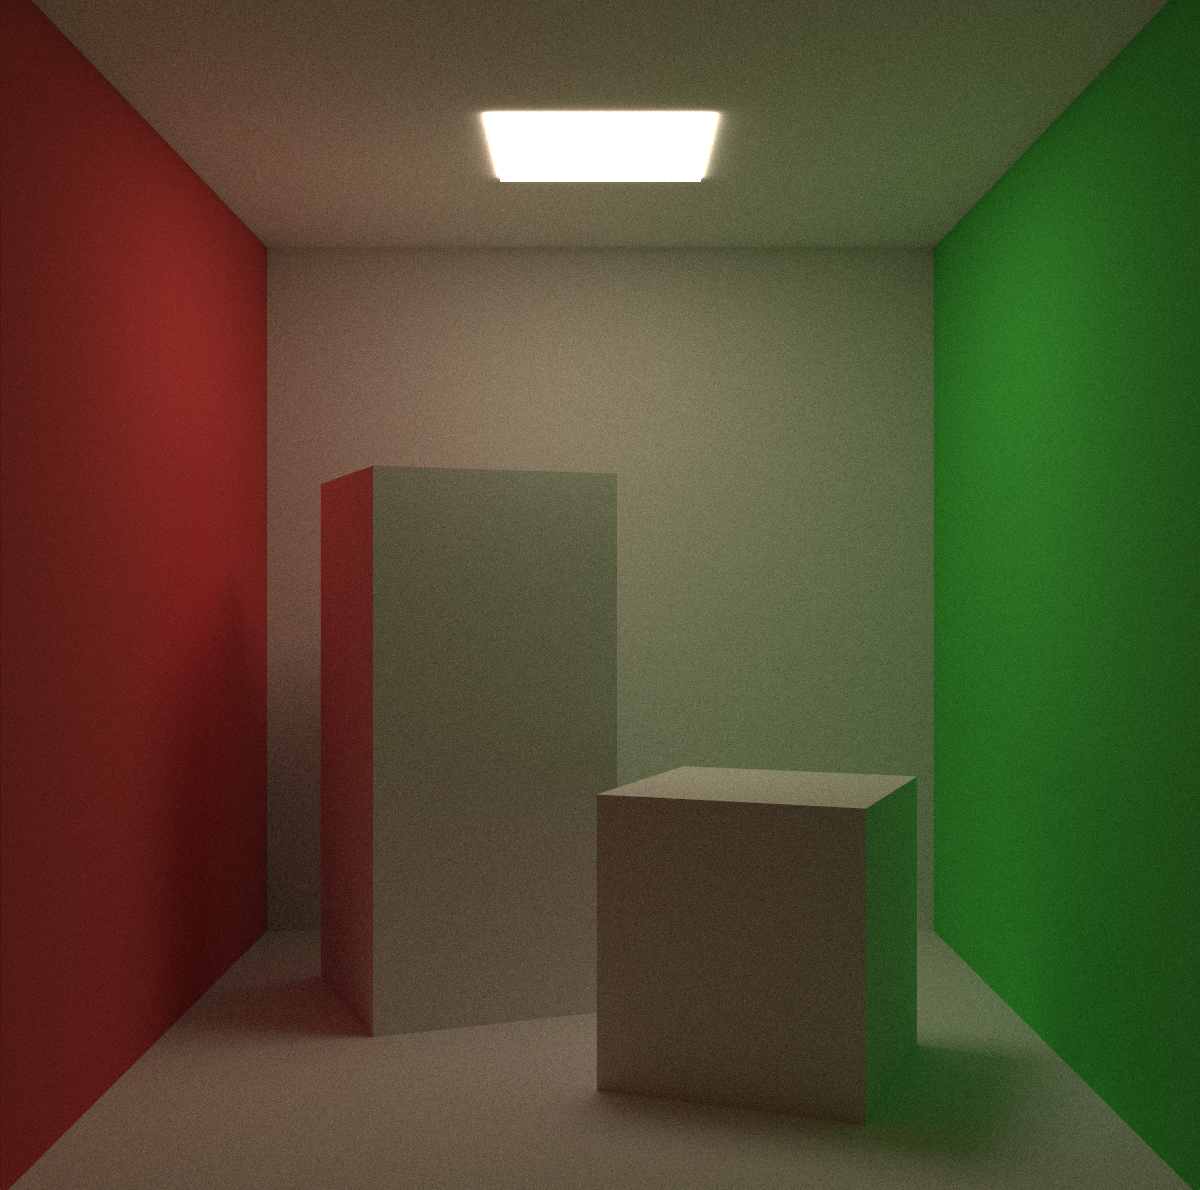
\includegraphics[width=\linewidth]{fig1.png}
        \caption{Green wall!}
    \end{subfigure}
    \begin{subfigure}{0.55\textwidth}
        \centering
        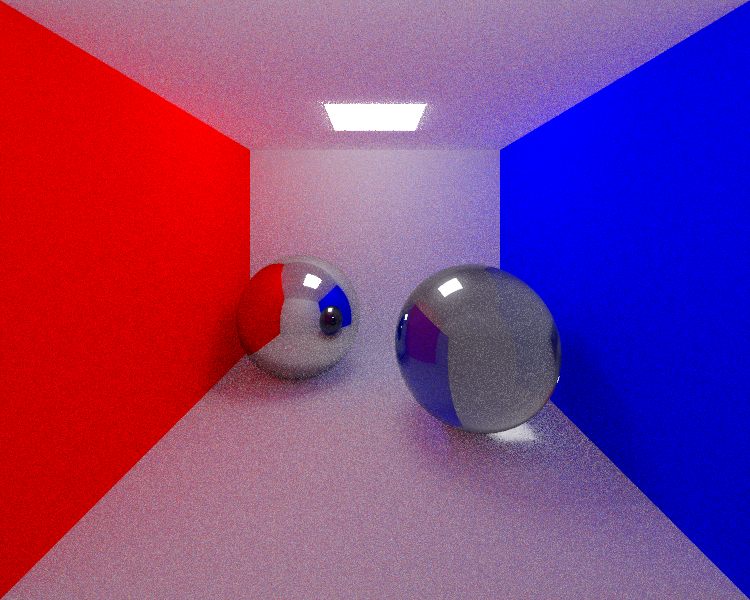
\includegraphics[width=\linewidth]{fig2.png}
        \caption{Blue wall!}
    \end{subfigure}
    \caption{Examples of Raytracing}
    \label{fig:fig1}
\end{figure}

\section{Optimizations in Ray Tracing}
\begin{enumerate}
    \item \textbf{Spatial Data Structures:}
    \begin{itemize}
        \item \textit{Bounding Volume Hierarchies (BVH):} \textcolor{blue}{BVH} is a widely-used method
        to reduce the number of ray-primitive intersection tests by organizing
        objects into hierarchical structures.
        \item \underline{\textcolor{red}{Kd-trees}} are also popular for partitioning 3D space to improve inter-
        section tests, particularly for static scenes.
    \end{itemize}
    \item \textbf{Acceleration Techniques:}
    \begin{itemize}
        \item[\textit{Ray Coherence:}] \textcolor{red}{Using coherent rays} helps in improving performance by ensuring sim-
        ilar rays follow the same code paths, enhancing cache efficiency.
        \item[\textit{Adaptive Sampling:}] Regions with high detail may use \textcolor{blue}{adaptive sampling} to concentrate
        more rays in critical areas, while flat regions use fewer rays, thereby
        reducing computation.
    \end{itemize}
\end{enumerate}
\printbibliography
\end{document}
